\documentclass{article}%
\usepackage[T1]{fontenc}%
\usepackage[utf8]{inputenc}%
\usepackage{lmodern}%
\usepackage{textcomp}%
\usepackage{lastpage}%
\usepackage[head=40pt,margin=0.5in,bottom=0.6in]{geometry}%
\usepackage{graphicx}%
%
\title{\textbf{Optan por quemar la basura ante fallas de aseo en Vargas}}%
\author{AMY TORRES}%
\date{26/11/2018}%
%
\begin{document}%
\normalsize%
\maketitle%
\textbf{URL: }%
http://www.eluniversal.com/caracas/26777/optan{-}por{-}quemar{-}la{-}basura{-}ante{-}fallas{-}de{-}aseo{-}en{-}vargas\newline%
%
\textbf{Periodico: }%
EU, %
ID: %
26777, %
Seccion: %
caracas\newline%
%
\textbf{Palabras Claves: }%
NO\_TIENE\newline%
%
\textbf{Derecho: }%
3.2%
, Otros Derechos: %
NO\_TIENE%
, Sub Derechos: %
3.2.1%
\newline%
%
\textbf{EP: }%
NO\newline%
\newline%
%
\textbf{\textit{Reportan que llevan semanas sin ver el camión de la basura por la zona.}}%
\newline%
\newline%
%
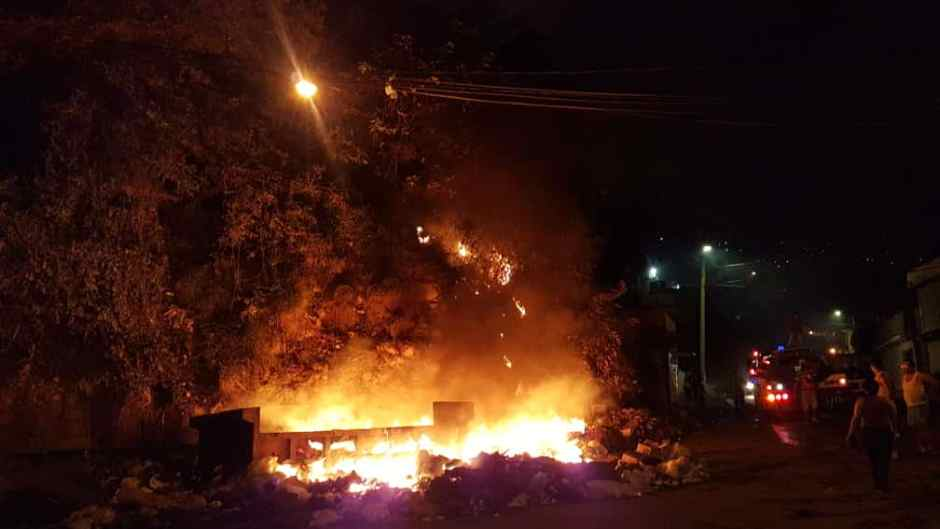
\includegraphics[width=300px]{252.jpg}%
\newline%
%
Calles abarrotadas de basura y vecinos inconscientes que siguen dejando sus bolsas en estos sitios públicos es el pan de cada día en comunidades del oeste y este de Vargas, que reportan semanas sin ver el aseo.%
\newline%
%
Tal es el caso de Guillermina Machado, residente de Las Tunitas, quien no solo se queja de la insalubridad producto de la acumulación de desperdicios, sino también por la escasez de gas.%
\newline%
%
En Marlboro, Carlos Soublette, “no se aguantan las moscas que atrae el mal olor del cuarto de basura. Aparte no tenemos agua y eso impide poder cumplir con el aseo de la casa como es debido”, denuncia Nellibe Hernández, quien también sostiene que hay fallas en la distribución de gas.%
\newline%
%
Debajo del puente de Caraballeda, en la avenida José María España, una nube de humo gris cubría la vía, y es que como última opción algunos vecinos están optando por quemar la basura a sabiendas incluso de que el remedio puede ser peor que la enfermedad.~Otros que se han visto obligados a hacerlo son residentes de El Brillante, en Maiquetía.%
\newline%
%
En Mamo hubo momentos de tensión el pasado viernes dado que también le prendieron fuego al contenedor de la zona, pero este se propagó a unas montañas aledañas lo que requirió la intervención de los Bomberos de Vargas.%
\newline%
%
Protestaron por agua en Mamo%
\newline%
%
Las fallas en los servicios públicos en el Litoral no solo tienen que ver con el de gas y de aseo, la falta de agua por tubería ha sido tradicionalmente una de las peores calamidades, solo que durante este último racionamiento hay comunidades que no gozan del servicio desde hace dos y tres meses.%
\newline%
%
Este lunes vecinos de Mamo tomaron la calle principal en reclamo por el vital líquido y en rechazo a las decenas de litros que se desperdician en el llenadero de Hidrocapital, en Mamo, cuando las familias deben pagar altos precios por llenar por lo menos un bidón.%
\newline%
%
\end{document}